\documentclass{standalone}
\usepackage{tikz}
\begin{document}

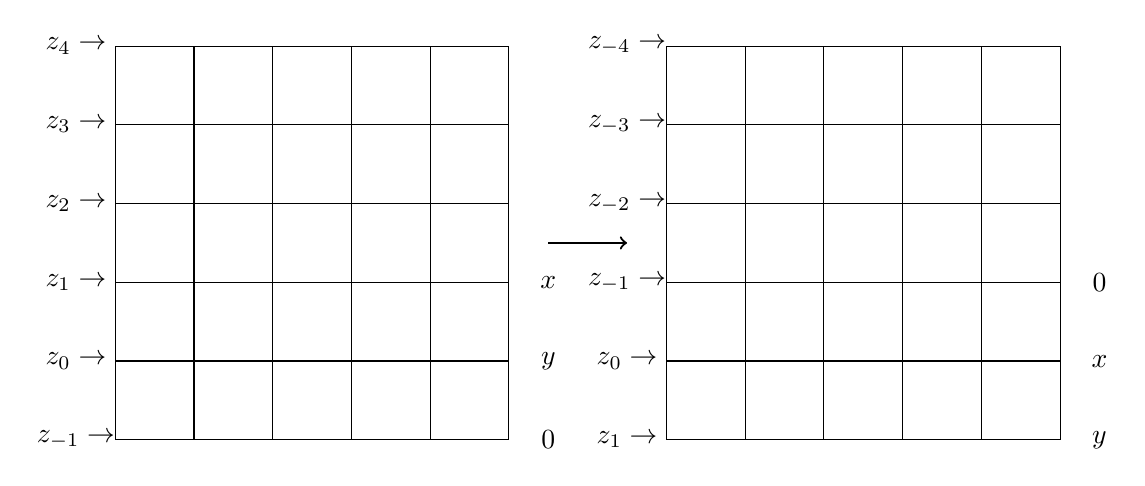
\begin{tikzpicture}

% First grid
\foreach \x in {0,1,...,5} {
    \draw (0,\x) -- (5,\x);
    \draw (\x,0) -- (\x,5);
}

% Labels for the first grid
\node at (-0.5,5) {$z_4 \to$};
\node at (-0.5,4) {$z_3 \to$};
\node at (-0.5,3) {$z_2 \to$};
\node at (-0.5,2) {$z_1 \to$};
\node at (-0.5,1) {$z_0 \to$};
\node at (-0.5,0) {$z_{-1} \to$};

\node at (5.5,2) {$x$};
\node at (5.5,1) {$y$};
\node at (5.5,0) {$0$};

% Arrow between grids
\draw[->, thick] (5.5,2.5) -- (6.5,2.5);

% Second grid
\foreach \x in {7,8,...,12} {
    \draw (\x,0) -- (\x,5);
    \draw (7,\x-7) -- (12,\x-7);
}

% Labels for the second grid
\node at (6.5,5) {$z_{-4} \to$};
\node at (6.5,4) {$z_{-3} \to$};
\node at (6.5,3) {$z_{-2} \to$};
\node at (6.5,2) {$z_{-1} \to$};
\node at (6.5,1) {$z_0 \to$};
\node at (6.5,0) {$z_1 \to$};

\node at (12.5,2) {$0$};
\node at (12.5,1) {$x$};
\node at (12.5,0) {$y$};

\end{tikzpicture}

\end{document}